\documentclass[border=10pt]{standalone}
\usepackage{tikz}\usepackage{amsmath}\usetikzlibrary{arrows.meta}
\begin{document}
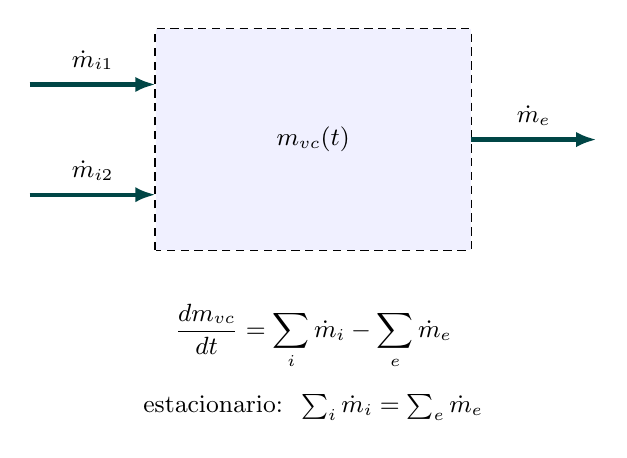
\begin{tikzpicture}[line width=1pt,>={Latex[length=2.6mm]}]
  \draw[densely dashed,line width=1.2pt] (0,0) rectangle (4.0,2.8);
  \fill[blue!6] (0,0) rectangle (4.0,2.8);
  \node[align=center] at (2.0,1.4){\small $m_{vc}(t)$};
  % entradas
  \draw[->,teal!55!black,line width=1.5pt] (-1.6,2.1)--(0,2.1); \node[above] at (-0.8,2.15){\small $\dot m_{i1}$};
  \draw[->,teal!55!black,line width=1.5pt] (-1.6,0.7)--(0,0.7); \node[above] at (-0.8,0.75){\small $\dot m_{i2}$};
  % salida
  \draw[->,teal!55!black,line width=1.5pt] (4.0,1.4)--(5.6,1.4); \node[above] at (4.8,1.45){\small $\dot m_{e}$};
  \node[align=center] at (2.0,-1.1){\small $\dfrac{dm_{vc}}{dt}=\displaystyle\sum_i \dot m_i-\sum_e \dot m_e$};
  \node[align=center] at (2.0,-2.0){\small estacionario:\; $\sum_i \dot m_i=\sum_e \dot m_e$};
\end{tikzpicture}
\end{document}
